% This file was converted from HTML to LaTeX with
% gnuhtml2latex program
% (c) Tomasz Wegrzanowski <maniek@beer.com> 1999
% (c) Gunnar Wolf <gwolf@gwolf.org> 2005-2010
% Version : 0.4.
\section{Laufen}
Auf dieser Seite wird die Movementklasse beschrieben, die dafür 
verantwortlich ist, dass der Nao sich zu einem Ziel bewegen kann. Wir 
haben beschlossen, die Laufbewegungen zu abstrahieren und verwenden 
stattdessen von der Simulation zur Verfügung gestellte Beam-Befehle.

\section{Aktueller Zustand}
In der aktuellen Implementation wird der Beam-Befehl für die 
Agentschnittstelle genutzt. Das heißt, es kann nach dem Anstoß nicht mehr genutzt werden. Außerdem steht uns die echte Position nicht zur 
Verfügung, die aber gebraucht wird, um sich realitätsnah zu bewegen. Zu 
diesem Zweck wird aktuell die Position in einer lokalen Variable 
gespeichert, was allerdings zu Problemen während des Spielverlaufs 
führen kann.\\
Obwohl sich der Nao langsam zu seinem Ziel drehen sollte, bevor er
 losgeht, wurde beschlossen damit zu warten, bis die echte Position 
verfügbar ist, da die vielen Workarounds die Funktion ohnehin schon 
Fehleranfällig machen. 

\section{Nutzung}
run(x,y)~: Rufe diese Funktion der Movementklasse auf, um einen 
Schritt in die Richtung des angegeben Zieles zu machen. x und y sind die
 Zielkoordinaten.

\section{Ansatz und Schnittstellen}
Es gibt zwei verschiedene Arten von Beam-Befehlen: \\
Über die Agent-Schnittstelle gibt es einen Beam-Befehl, um die 
Naos vor dem Anstoß zu positionieren. Nach dem Anstoß wird diese 
Schnittstelle nicht mehr funktionieren, deswegen ist diese Schnittstelle 
nicht möglich.\\
Über das Monitor-Protokoll gibt es ebenfalls mehrere 
Beam-Befehle. Diese sind eigentlich für den Schiedsrichter oder 
ähnliches gedacht und können deshalb auch nach dem Anpfiff genutzt 
werden. Dieses soll am Ende genutzt werden.\\
Da alle Beam-Befehle mit absoluten Variablen arbeiten, benötigen 
wir unsere echte Position, um den nächsten Schritt (der natürlich 
mithilfe der Wahrnehmung berechnet werden soll) relativ zu unserer 
Position ausgeführt werden kann.

\section{Berechnungen}
Um uns dem Ziel zu nähern, berechnen wir den Winkel in dem das Ziel von 
der aktuellen Position aus liegt und bewegen uns einen Schritt in diese 
Richtung. \\   
Wenn (a, b) die aktuelle Position ist und (c, d) die Zielkoordinaten, dann berechnen wir den Winkel mit folgender Formel:\\
\begin{equation}
angle = arctan \frac{c - a}{d -b}
\end{equation}
\begin{figure}
\begin{center}
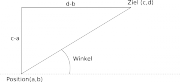
\includegraphics[scale=1]{180px-Winkel}
\end{center}
\caption{Winkelberechnung}
\end{figure}
\begin{figure}
\begin{center}
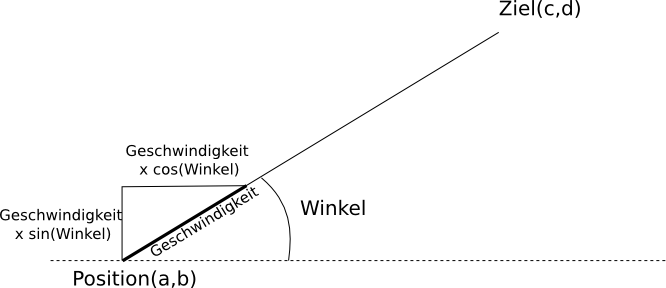
\includegraphics[scale=0.6]{geschwindigkeit}
\end{center}
\caption{Berechnung des nächsten Schrittes}
\end{figure}
Wir verwenden die Funktion atan2 von Python, die es ermöglicht 
zwei Argumente zu übergeben ohne die Division, so dass der eindeutige 
Winkel berechnet werden kann.\\
Danach wird Sinus und Kosinus des Winkels berechnet, mit der 
Geschwindigkeit multipliziert und auf die entsprechenden 
Positionskoordinaten aufsummiert, um eine einheitliche Schrittlänge zu 
gewährleisten.\\
Der Winkel muss vor dem Übergeben an die Simulation zu Grad 
konvertiert, negiert und um $90^\circ$ $(n/2)$ erhöht werden damit er mit den, 
von simspark erwarteten Werten, übereinstimmt.\\
Danach wird die neue Position, sowie der berechnete Winkel in einem Beam-Befehl übergeben.

\section{Protokoll}
Der Beam-Befehl über die Agenten-Schnittstelle nimmt die folgende Form an:

\begin{verbatim}(beam <x> <y> <rot>)
\end{verbatim}
Wobei x und y die entsprechenden Koordinaten sind und $<$rot$>$ der
 Winkel, in den der Nao schauen soll. Dieser Ansatz soll später durch das Monitorprotokoll ersetzt 
werden.\\
Im Monitorprotokoll gibt es ein Befehl, mit dem man einen einzelnen Nao bearbeiten kann:

\begin{verbatim}(agent (unum <num>) (team <team>) (pos <x> <y> <z>)
                                  (move <x> <y> <z> <rot>)
                                  (battery <batterylevel>)
                                  (temperature <temperature>)
)
\end{verbatim}
Da dieser Befehl normalerweise nicht vom Nao kommt sondern vom 
Schiedsrichter oder ähnliches, muss hier sowohl das Team als auch die 
Spielernummer mit angegeben werden. Da wir auch die Rotation mit angeben
 wollen werden wir auf den move-Abschnitt des Befehls zurückgreifen. pos
 battery und temperature können weggelassen werden, wenn sie nicht 
genutzt werden.\\
Alle Argumente müssen absolut abgegeben werden.
